\documentclass[1p]{elsarticle_modified}
%\bibliographystyle{elsarticle-num}

%\usepackage[colorlinks]{hyperref}
%\usepackage{abbrmath_seonhwa} %\Abb, \Ascr, \Acal ,\Abf, \Afrak
\usepackage{amsfonts}
\usepackage{amssymb}
\usepackage{amsmath}
\usepackage{amsthm}
\usepackage{scalefnt}
\usepackage{amsbsy}
\usepackage{kotex}
\usepackage{caption}
\usepackage{subfig}
\usepackage{color}
\usepackage{graphicx}
\usepackage{xcolor} %% white, black, red, green, blue, cyan, magenta, yellow
\usepackage{float}
\usepackage{setspace}
\usepackage{hyperref}

\usepackage{tikz}
\usetikzlibrary{arrows}

\usepackage{multirow}
\usepackage{array} % fixed length table
\usepackage{hhline}

%%%%%%%%%%%%%%%%%%%%%
\makeatletter
\renewcommand*\env@matrix[1][\arraystretch]{%
	\edef\arraystretch{#1}%
	\hskip -\arraycolsep
	\let\@ifnextchar\new@ifnextchar
	\array{*\c@MaxMatrixCols c}}
\makeatother %https://tex.stackexchange.com/questions/14071/how-can-i-increase-the-line-spacing-in-a-matrix
%%%%%%%%%%%%%%%

\usepackage[normalem]{ulem}

\newcommand{\msout}[1]{\ifmmode\text{\sout{\ensuremath{#1}}}\else\sout{#1}\fi}
%SOURCE: \msout is \stkout macro in https://tex.stackexchange.com/questions/20609/strikeout-in-math-mode

\newcommand{\cancel}[1]{
	\ifmmode
	{\color{red}\msout{#1}}
	\else
	{\color{red}\sout{#1}}
	\fi
}

\newcommand{\add}[1]{
	{\color{blue}\uwave{#1}}
}

\newcommand{\replace}[2]{
	\ifmmode
	{\color{red}\msout{#1}}{\color{blue}\uwave{#2}}
	\else
	{\color{red}\sout{#1}}{\color{blue}\uwave{#2}}
	\fi
}

\newcommand{\Sol}{\mathcal{S}} %segment
\newcommand{\D}{D} %diagram
\newcommand{\A}{\mathcal{A}} %arc


%%%%%%%%%%%%%%%%%%%%%%%%%%%%%5 test

\def\sl{\operatorname{\textup{SL}}(2,\Cbb)}
\def\psl{\operatorname{\textup{PSL}}(2,\Cbb)}
\def\quan{\mkern 1mu \triangleright \mkern 1mu}

\theoremstyle{definition}
\newtheorem{thm}{Theorem}[section]
\newtheorem{prop}[thm]{Proposition}
\newtheorem{lem}[thm]{Lemma}
\newtheorem{ques}[thm]{Question}
\newtheorem{cor}[thm]{Corollary}
\newtheorem{defn}[thm]{Definition}
\newtheorem{exam}[thm]{Example}
\newtheorem{rmk}[thm]{Remark}
\newtheorem{alg}[thm]{Algorithm}

\newcommand{\I}{\sqrt{-1}}
\begin{document}

%\begin{frontmatter}
%
%\title{Boundary parabolic representations of knots up to 8 crossings}
%
%%% Group authors per affiliation:
%\author{Yunhi Cho} 
%\address{Department of Mathematics, University of Seoul, Seoul, Korea}
%\ead{yhcho@uos.ac.kr}
%
%
%\author{Seonhwa Kim} %\fnref{s_kim}}
%\address{Center for Geometry and Physics, Institute for Basic Science, Pohang, 37673, Korea}
%\ead{ryeona17@ibs.re.kr}
%
%\author{Hyuk Kim}
%\address{Department of Mathematical Sciences, Seoul National University, Seoul 08826, Korea}
%\ead{hyukkim@snu.ac.kr}
%
%\author{Seokbeom Yoon}
%\address{Department of Mathematical Sciences, Seoul National University, Seoul, 08826,  Korea}
%\ead{sbyoon15@snu.ac.kr}
%
%\begin{abstract}
%We find all boundary parabolic representation of knots up to 8 crossings.
%
%\end{abstract}
%\begin{keyword}
%    \MSC[2010] 57M25 
%\end{keyword}
%
%\end{frontmatter}

%\linenumbers
%\tableofcontents
%
\newcommand\colored[1]{\textcolor{white}{\rule[-0.35ex]{0.8em}{1.4ex}}\kern-0.8em\color{red} #1}%
%\newcommand\colored[1]{\textcolor{white}{ #1}\kern-2.17ex	\textcolor{white}{ #1}\kern-1.81ex	\textcolor{white}{ #1}\kern-2.15ex\color{red}#1	}

{\Large $\underline{12a_{0511}~(K12a_{0511})}$}

\setlength{\tabcolsep}{10pt}
\renewcommand{\arraystretch}{1.6}
\vspace{1cm}\begin{tabular}{m{100pt}>{\centering\arraybackslash}m{274pt}}
\multirow{5}{120pt}{
	\centering
	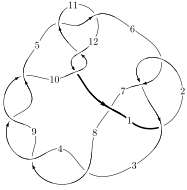
\includegraphics[width=112pt]{../../../GIT/diagram.site/Diagrams/png/1312_12a_0511.png}\\
\ \ \ A knot diagram\footnotemark}&
\allowdisplaybreaks
\textbf{Linearized knot diagam} \\
\cline{2-2}
 &
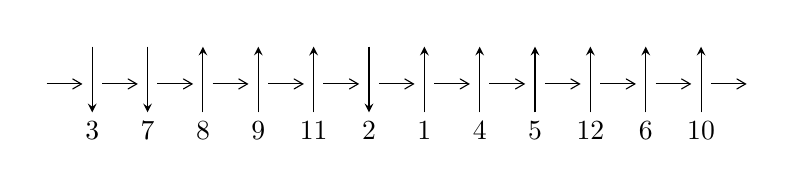
\begin{tikzpicture}[x=20pt, y=17pt]
	% nodes
	\node (C0) at (0, 0) {};
	\node (C1) at (1, 0) {};
	\node (C1U) at (1, +1) {};
	\node (C1D) at (1, -1) {3};

	\node (C2) at (2, 0) {};
	\node (C2U) at (2, +1) {};
	\node (C2D) at (2, -1) {7};

	\node (C3) at (3, 0) {};
	\node (C3U) at (3, +1) {};
	\node (C3D) at (3, -1) {8};

	\node (C4) at (4, 0) {};
	\node (C4U) at (4, +1) {};
	\node (C4D) at (4, -1) {9};

	\node (C5) at (5, 0) {};
	\node (C5U) at (5, +1) {};
	\node (C5D) at (5, -1) {11};

	\node (C6) at (6, 0) {};
	\node (C6U) at (6, +1) {};
	\node (C6D) at (6, -1) {2};

	\node (C7) at (7, 0) {};
	\node (C7U) at (7, +1) {};
	\node (C7D) at (7, -1) {1};

	\node (C8) at (8, 0) {};
	\node (C8U) at (8, +1) {};
	\node (C8D) at (8, -1) {4};

	\node (C9) at (9, 0) {};
	\node (C9U) at (9, +1) {};
	\node (C9D) at (9, -1) {5};

	\node (C10) at (10, 0) {};
	\node (C10U) at (10, +1) {};
	\node (C10D) at (10, -1) {12};

	\node (C11) at (11, 0) {};
	\node (C11U) at (11, +1) {};
	\node (C11D) at (11, -1) {6};

	\node (C12) at (12, 0) {};
	\node (C12U) at (12, +1) {};
	\node (C12D) at (12, -1) {10};
	\node (C13) at (13, 0) {};

	% arrows
	\draw[->,>={angle 60}]
	(C0) edge (C1) (C1) edge (C2) (C2) edge (C3) (C3) edge (C4) (C4) edge (C5) (C5) edge (C6) (C6) edge (C7) (C7) edge (C8) (C8) edge (C9) (C9) edge (C10) (C10) edge (C11) (C11) edge (C12) (C12) edge (C13) ;	\draw[->,>=stealth]
	(C1U) edge (C1D) (C2U) edge (C2D) (C3D) edge (C3U) (C4D) edge (C4U) (C5D) edge (C5U) (C6U) edge (C6D) (C7D) edge (C7U) (C8D) edge (C8U) (C9D) edge (C9U) (C10D) edge (C10U) (C11D) edge (C11U) (C12D) edge (C12U) ;
	\end{tikzpicture} \\
\hhline{~~} \\& 
\textbf{Solving Sequence} \\ \cline{2-2} 
 &
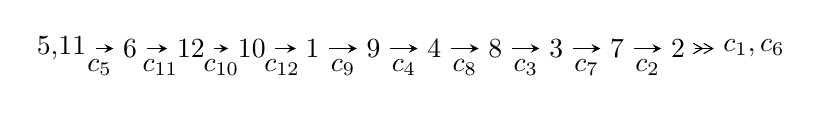
\begin{tikzpicture}[x=22pt, y=7pt]
	% node
	\node (A0) at (-1/8, 0) {5,11};
	\node (A1) at (1, 0) {6};
	\node (A2) at (2, 0) {12};
	\node (A3) at (3, 0) {10};
	\node (A4) at (4, 0) {1};
	\node (A5) at (5, 0) {9};
	\node (A6) at (6, 0) {4};
	\node (A7) at (7, 0) {8};
	\node (A8) at (8, 0) {3};
	\node (A9) at (9, 0) {7};
	\node (A10) at (10, 0) {2};
	\node (C1) at (1/2, -1) {$c_{5}$};
	\node (C2) at (3/2, -1) {$c_{11}$};
	\node (C3) at (5/2, -1) {$c_{10}$};
	\node (C4) at (7/2, -1) {$c_{12}$};
	\node (C5) at (9/2, -1) {$c_{9}$};
	\node (C6) at (11/2, -1) {$c_{4}$};
	\node (C7) at (13/2, -1) {$c_{8}$};
	\node (C8) at (15/2, -1) {$c_{3}$};
	\node (C9) at (17/2, -1) {$c_{7}$};
	\node (C10) at (19/2, -1) {$c_{2}$};
	\node (A11) at (45/4, 0) {$c_{1},c_{6}$};

	% edge
	\draw[->,>=stealth]	
	(A0) edge (A1) (A1) edge (A2) (A2) edge (A3) (A3) edge (A4) (A4) edge (A5) (A5) edge (A6) (A6) edge (A7) (A7) edge (A8) (A8) edge (A9) (A9) edge (A10) ;
	\draw[->>,>={angle 60}]	
	(A10) edge (A11);
\end{tikzpicture} \\ 

\end{tabular} \\

\footnotetext{
The image of knot diagram is generated by the software ``\textbf{Draw programme}" developed by Andrew Bartholomew(\url{http://www.layer8.co.uk/maths/draw/index.htm\#Running-draw}), where we modified some parts for our purpose(\url{https://github.com/CATsTAILs/LinksPainter}).
}\phantom \\ \newline 
\centering \textbf{Ideals for irreducible components\footnotemark of $X_{\text{par}}$} 
 
\begin{align*}
I^u_{1}&=\langle 
u^{52}- u^{51}+\cdots- u^2+1\rangle \\
I^u_{2}&=\langle 
u^{10}-2 u^8+3 u^6+u^5-2 u^4- u^3+u^2+u-1\rangle \\
\\
\end{align*}
\raggedright * 2 irreducible components of $\dim_{\mathbb{C}}=0$, with total 62 representations.\\
\footnotetext{All coefficients of polynomials are rational numbers. But the coefficients are sometimes approximated in decimal forms when there is not enough margin.}
\newpage
\renewcommand{\arraystretch}{1}
\centering \section*{I. $I^u_{1}= \langle u^{52}- u^{51}+\cdots- u^2+1 \rangle$}
\flushleft \textbf{(i) Arc colorings}\\
\begin{tabular}{m{7pt} m{180pt} m{7pt} m{180pt} }
\flushright $a_{5}=$&$\begin{pmatrix}1\\0\end{pmatrix}$ \\
\flushright $a_{11}=$&$\begin{pmatrix}0\\u\end{pmatrix}$ \\
\flushright $a_{6}=$&$\begin{pmatrix}1\\- u^2\end{pmatrix}$ \\
\flushright $a_{12}=$&$\begin{pmatrix}u\\- u^3+u\end{pmatrix}$ \\
\flushright $a_{10}=$&$\begin{pmatrix}- u^3\\u^5- u^3+u\end{pmatrix}$ \\
\flushright $a_{1}=$&$\begin{pmatrix}u^5+u\\- u^7+u^5-2 u^3+u\end{pmatrix}$ \\
\flushright $a_{9}=$&$\begin{pmatrix}- u^5- u\\u^5- u^3+u\end{pmatrix}$ \\
\flushright $a_{4}=$&$\begin{pmatrix}- u^{10}+u^8-2 u^6+u^4- u^2+1\\u^{10}-2 u^8+3 u^6-2 u^4+u^2\end{pmatrix}$ \\
\flushright $a_{8}=$&$\begin{pmatrix}u^{15}-2 u^{13}+4 u^{11}-4 u^9+4 u^7-4 u^5+2 u^3-2 u\\- u^{15}+3 u^{13}-6 u^{11}+7 u^9-6 u^7+4 u^5-2 u^3+u\end{pmatrix}$ \\
\flushright $a_{3}=$&$\begin{pmatrix}u^{20}-3 u^{18}+\cdots-3 u^2+1\\- u^{20}+4 u^{18}+\cdots-5 u^4+2 u^2\end{pmatrix}$ \\
\flushright $a_{7}=$&$\begin{pmatrix}- u^{27}+4 u^{25}+\cdots- u^3-2 u\\u^{29}-5 u^{27}+\cdots-5 u^3+u\end{pmatrix}$ \\
\flushright $a_{2}=$&$\begin{pmatrix}u^{47}-8 u^{45}+\cdots-42 u^5+10 u^3\\- u^{47}+9 u^{45}+\cdots-4 u^3+u\end{pmatrix}$\\&\end{tabular}
\flushleft \textbf{(ii) Obstruction class $= -1$}\\~\\
\flushleft \textbf{(iii) Cusp Shapes $= -4 u^{51}+40 u^{49}+\cdots+16 u+10$}\\~\\
\newpage\renewcommand{\arraystretch}{1}
\flushleft \textbf{(iv) u-Polynomials at the component}\newline \\
\begin{tabular}{m{50pt}|m{274pt}}
Crossings & \hspace{64pt}u-Polynomials at each crossing \\
\hline $$\begin{aligned}c_{1}\end{aligned}$$&$\begin{aligned}
&u^{52}+23 u^{51}+\cdots+2 u+1
\end{aligned}$\\
\hline $$\begin{aligned}c_{2},c_{6}\end{aligned}$$&$\begin{aligned}
&u^{52}- u^{51}+\cdots-2 u+1
\end{aligned}$\\
\hline $$\begin{aligned}c_{3},c_{4},c_{8}\\c_{9}\end{aligned}$$&$\begin{aligned}
&u^{52}-4 u^{51}+\cdots+36 u+4
\end{aligned}$\\
\hline $$\begin{aligned}c_{5},c_{11}\end{aligned}$$&$\begin{aligned}
&u^{52}- u^{51}+\cdots- u^2+1
\end{aligned}$\\
\hline $$\begin{aligned}c_{7}\end{aligned}$$&$\begin{aligned}
&u^{52}-3 u^{51}+\cdots-8 u+5
\end{aligned}$\\
\hline $$\begin{aligned}c_{10},c_{12}\end{aligned}$$&$\begin{aligned}
&u^{52}-19 u^{51}+\cdots-2 u+1
\end{aligned}$\\
\hline
\end{tabular}\\~\\
\newpage\renewcommand{\arraystretch}{1}
\flushleft \textbf{(v) Riley Polynomials at the component}\newline \\
\begin{tabular}{m{50pt}|m{274pt}}
Crossings & \hspace{64pt}Riley Polynomials at each crossing \\
\hline $$\begin{aligned}c_{1}\end{aligned}$$&$\begin{aligned}
&y^{52}+13 y^{51}+\cdots-6 y+1
\end{aligned}$\\
\hline $$\begin{aligned}c_{2},c_{6}\end{aligned}$$&$\begin{aligned}
&y^{52}-23 y^{51}+\cdots-2 y+1
\end{aligned}$\\
\hline $$\begin{aligned}c_{3},c_{4},c_{8}\\c_{9}\end{aligned}$$&$\begin{aligned}
&y^{52}-60 y^{51}+\cdots-696 y+16
\end{aligned}$\\
\hline $$\begin{aligned}c_{5},c_{11}\end{aligned}$$&$\begin{aligned}
&y^{52}-19 y^{51}+\cdots-2 y+1
\end{aligned}$\\
\hline $$\begin{aligned}c_{7}\end{aligned}$$&$\begin{aligned}
&y^{52}-3 y^{51}+\cdots-534 y+25
\end{aligned}$\\
\hline $$\begin{aligned}c_{10},c_{12}\end{aligned}$$&$\begin{aligned}
&y^{52}+29 y^{51}+\cdots-6 y+1
\end{aligned}$\\
\hline
\end{tabular}\\~\\
\newpage\flushleft \textbf{(vi) Complex Volumes and Cusp Shapes}
$$\begin{array}{c|c|c}  
\text{Solutions to }I^u_{1}& \I (\text{vol} + \sqrt{-1}CS) & \text{Cusp shape}\\
 \hline 
\begin{aligned}
u &= -0.998941 + 0.045978 I\end{aligned}
 & \phantom{-}5.28620 - 0.93871 I & \phantom{-}15.9673 + 0.9512 I \\ \hline\begin{aligned}
u &= -0.998941 - 0.045978 I\end{aligned}
 & \phantom{-}5.28620 + 0.93871 I & \phantom{-}15.9673 - 0.9512 I \\ \hline\begin{aligned}
u &= -0.728323 + 0.685940 I\end{aligned}
 & -3.57521 - 0.97987 I & \phantom{-}0.260565 + 0.640305 I \\ \hline\begin{aligned}
u &= -0.728323 - 0.685940 I\end{aligned}
 & -3.57521 + 0.97987 I & \phantom{-}0.260565 - 0.640305 I \\ \hline\begin{aligned}
u &= \phantom{-}1.002230 + 0.089379 I\end{aligned}
 & \phantom{-}3.67626 + 5.72177 I & \phantom{-}12.7013 - 6.5868 I \\ \hline\begin{aligned}
u &= \phantom{-}1.002230 - 0.089379 I\end{aligned}
 & \phantom{-}3.67626 - 5.72177 I & \phantom{-}12.7013 + 6.5868 I \\ \hline\begin{aligned}
u &= -0.665641 + 0.720471 I\end{aligned}
 & -1.78289 + 5.70739 I & \phantom{-}3.97022 - 5.89201 I \\ \hline\begin{aligned}
u &= -0.665641 - 0.720471 I\end{aligned}
 & -1.78289 - 5.70739 I & \phantom{-}3.97022 + 5.89201 I \\ \hline\begin{aligned}
u &= \phantom{-}0.530837 + 0.816404 I\end{aligned}
 & \phantom{-}6.92563 - 8.79045 I & \phantom{-}7.25155 + 4.85962 I \\ \hline\begin{aligned}
u &= \phantom{-}0.530837 - 0.816404 I\end{aligned}
 & \phantom{-}6.92563 + 8.79045 I & \phantom{-}7.25155 - 4.85962 I \\ \hline\begin{aligned}
u &= -0.522819 + 0.813333 I\end{aligned}
 & \phantom{-}8.75278 + 3.37930 I & \phantom{-}9.83163 - 0.35758 I \\ \hline\begin{aligned}
u &= -0.522819 - 0.813333 I\end{aligned}
 & \phantom{-}8.75278 - 3.37930 I & \phantom{-}9.83163 + 0.35758 I \\ \hline\begin{aligned}
u &= \phantom{-}0.521713 + 0.791233 I\end{aligned}
 & \phantom{-}3.07937 - 1.57482 I & \phantom{-}4.02266 + 0.18175 I \\ \hline\begin{aligned}
u &= \phantom{-}0.521713 - 0.791233 I\end{aligned}
 & \phantom{-}3.07937 + 1.57482 I & \phantom{-}4.02266 - 0.18175 I \\ \hline\begin{aligned}
u &= -0.833280 + 0.443412 I\end{aligned}
 & \phantom{-}0.09032 - 4.10436 I & \phantom{-}9.88532 + 7.11286 I \\ \hline\begin{aligned}
u &= -0.833280 - 0.443412 I\end{aligned}
 & \phantom{-}0.09032 + 4.10436 I & \phantom{-}9.88532 - 7.11286 I \\ \hline\begin{aligned}
u &= \phantom{-}0.650819 + 0.682385 I\end{aligned}
 & \phantom{-}0.204162 - 1.159700 I & \phantom{-}7.88295 + 1.51609 I \\ \hline\begin{aligned}
u &= \phantom{-}0.650819 - 0.682385 I\end{aligned}
 & \phantom{-}0.204162 + 1.159700 I & \phantom{-}7.88295 - 1.51609 I \\ \hline\begin{aligned}
u &= \phantom{-}0.492028 + 0.801217 I\end{aligned}
 & \phantom{-}7.16166 + 5.41348 I & \phantom{-}7.59584 - 4.65169 I \\ \hline\begin{aligned}
u &= \phantom{-}0.492028 - 0.801217 I\end{aligned}
 & \phantom{-}7.16166 - 5.41348 I & \phantom{-}7.59584 + 4.65169 I \\ \hline\begin{aligned}
u &= -0.850769 + 0.649712 I\end{aligned}
 & -2.04278 - 2.52764 I & \phantom{-}4.28217 + 3.73621 I \\ \hline\begin{aligned}
u &= -0.850769 - 0.649712 I\end{aligned}
 & -2.04278 + 2.52764 I & \phantom{-}4.28217 - 3.73621 I \\ \hline\begin{aligned}
u &= \phantom{-}0.823932 + 0.690742 I\end{aligned}
 & -4.74803 - 0.75860 I & -0.678268 + 1.202668 I \\ \hline\begin{aligned}
u &= \phantom{-}0.823932 - 0.690742 I\end{aligned}
 & -4.74803 + 0.75860 I & -0.678268 - 1.202668 I \\ \hline\begin{aligned}
u &= \phantom{-}0.874578 + 0.686205 I\end{aligned}
 & -4.59465 + 6.05228 I & \phantom{-0.000000 } 0. - 7.84880 I \\ \hline\begin{aligned}
u &= \phantom{-}0.874578 - 0.686205 I\end{aligned}
 & -4.59465 - 6.05228 I & \phantom{-0.000000 -}0. + 7.84880 I \\ \hline\begin{aligned}
u &= \phantom{-}0.982865 + 0.602859 I\end{aligned}
 & \phantom{-}2.10133 + 4.69499 I & \phantom{-}11.88053 - 6.10182 I \\ \hline\begin{aligned}
u &= \phantom{-}0.982865 - 0.602859 I\end{aligned}
 & \phantom{-}2.10133 - 4.69499 I & \phantom{-}11.88053 + 6.10182 I \\ \hline\begin{aligned}
u &= -0.946937 + 0.662515 I\end{aligned}
 & -2.91580 - 4.23415 I & \phantom{-0.000000 -}0. + 5.26094 I \\ \hline\begin{aligned}
u &= -0.946937 - 0.662515 I\end{aligned}
 & -2.91580 + 4.23415 I & \phantom{-0.000000 } 0. - 5.26094 I\\
 \hline 
 \end{array}$$\newpage$$\begin{array}{c|c|c}  
\text{Solutions to }I^u_{1}& \I (\text{vol} + \sqrt{-1}CS) & \text{Cusp shape}\\
 \hline 
\begin{aligned}
u &= -1.158760 + 0.014478 I\end{aligned}
 & \phantom{-}12.9367 - 7.2052 I & \phantom{-}13.29023 + 4.77271 I \\ \hline\begin{aligned}
u &= -1.158760 - 0.014478 I\end{aligned}
 & \phantom{-}12.9367 + 7.2052 I & \phantom{-}13.29023 - 4.77271 I \\ \hline\begin{aligned}
u &= \phantom{-}1.159210 + 0.007998 I\end{aligned}
 & \phantom{-}14.7139 + 1.7466 I & \phantom{-}15.7254 + 0. I\phantom{ +0.000000I} \\ \hline\begin{aligned}
u &= \phantom{-}1.159210 - 0.007998 I\end{aligned}
 & \phantom{-}14.7139 - 1.7466 I & \phantom{-}15.7254 + 0. I\phantom{ +0.000000I} \\ \hline\begin{aligned}
u &= \phantom{-}0.984648 + 0.652855 I\end{aligned}
 & \phantom{-}1.18503 + 6.34235 I & \phantom{-}6.00000 - 6.57485 I \\ \hline\begin{aligned}
u &= \phantom{-}0.984648 - 0.652855 I\end{aligned}
 & \phantom{-}1.18503 - 6.34235 I & \phantom{-}6.00000 + 6.57485 I \\ \hline\begin{aligned}
u &= -0.986168 + 0.671138 I\end{aligned}
 & -0.83243 - 11.04580 I & \phantom{-0.000000 -}0. + 10.84993 I \\ \hline\begin{aligned}
u &= -0.986168 - 0.671138 I\end{aligned}
 & -0.83243 + 11.04580 I & \phantom{-0.000000 } 0. - 10.84993 I \\ \hline\begin{aligned}
u &= \phantom{-}1.064000 + 0.654185 I\end{aligned}
 & \phantom{-}4.67776 + 7.01331 I & \phantom{-0.000000 } 0 \\ \hline\begin{aligned}
u &= \phantom{-}1.064000 - 0.654185 I\end{aligned}
 & \phantom{-}4.67776 - 7.01331 I & \phantom{-0.000000 } 0 \\ \hline\begin{aligned}
u &= -1.074140 + 0.648969 I\end{aligned}
 & \phantom{-}10.57820 - 5.44672 I & \phantom{-0.000000 } 0 \\ \hline\begin{aligned}
u &= -1.074140 - 0.648969 I\end{aligned}
 & \phantom{-}10.57820 + 5.44672 I & \phantom{-0.000000 } 0 \\ \hline\begin{aligned}
u &= -1.072330 + 0.660031 I\end{aligned}
 & \phantom{-}10.38760 - 8.89731 I & \phantom{-0.000000 } 0 \\ \hline\begin{aligned}
u &= -1.072330 - 0.660031 I\end{aligned}
 & \phantom{-}10.38760 + 8.89731 I & \phantom{-0.000000 } 0 \\ \hline\begin{aligned}
u &= \phantom{-}1.071430 + 0.664123 I\end{aligned}
 & \phantom{-}8.5369 + 14.3344 I & \phantom{-0.000000 } 0 \\ \hline\begin{aligned}
u &= \phantom{-}1.071430 - 0.664123 I\end{aligned}
 & \phantom{-}8.5369 - 14.3344 I & \phantom{-0.000000 } 0 \\ \hline\begin{aligned}
u &= \phantom{-}0.649830 + 0.190765 I\end{aligned}
 & \phantom{-}0.943472 + 0.087273 I & \phantom{-}11.64609 - 1.04296 I \\ \hline\begin{aligned}
u &= \phantom{-}0.649830 - 0.190765 I\end{aligned}
 & \phantom{-}0.943472 - 0.087273 I & \phantom{-}11.64609 + 1.04296 I \\ \hline\begin{aligned}
u &= -0.355914 + 0.492873 I\end{aligned}
 & -0.32921 - 4.26537 I & \phantom{-}5.60545 + 7.03160 I \\ \hline\begin{aligned}
u &= -0.355914 - 0.492873 I\end{aligned}
 & -0.32921 + 4.26537 I & \phantom{-}5.60545 - 7.03160 I \\ \hline\begin{aligned}
u &= -0.114095 + 0.393922 I\end{aligned}
 & -1.45941 + 1.41253 I & \phantom{-}0.827325 - 0.785575 I \\ \hline\begin{aligned}
u &= -0.114095 - 0.393922 I\end{aligned}
 & -1.45941 - 1.41253 I & \phantom{-}0.827325 + 0.785575 I\\
 \hline 
 \end{array}$$\newpage\newpage\renewcommand{\arraystretch}{1}
\centering \section*{II. $I^u_{2}= \langle u^{10}-2 u^8+3 u^6+u^5-2 u^4- u^3+u^2+u-1 \rangle$}
\flushleft \textbf{(i) Arc colorings}\\
\begin{tabular}{m{7pt} m{180pt} m{7pt} m{180pt} }
\flushright $a_{5}=$&$\begin{pmatrix}1\\0\end{pmatrix}$ \\
\flushright $a_{11}=$&$\begin{pmatrix}0\\u\end{pmatrix}$ \\
\flushright $a_{6}=$&$\begin{pmatrix}1\\- u^2\end{pmatrix}$ \\
\flushright $a_{12}=$&$\begin{pmatrix}u\\- u^3+u\end{pmatrix}$ \\
\flushright $a_{10}=$&$\begin{pmatrix}- u^3\\u^5- u^3+u\end{pmatrix}$ \\
\flushright $a_{1}=$&$\begin{pmatrix}u^5+u\\- u^7+u^5-2 u^3+u\end{pmatrix}$ \\
\flushright $a_{9}=$&$\begin{pmatrix}- u^5- u\\u^5- u^3+u\end{pmatrix}$ \\
\flushright $a_{4}=$&$\begin{pmatrix}- u^8+u^6+u^5- u^4- u^3+u\\- u^5+u^3- u+1\end{pmatrix}$ \\
\flushright $a_{8}=$&$\begin{pmatrix}- u^8+u^6- u^4-1\\- u^5+u^3- u+1\end{pmatrix}$ \\
\flushright $a_{3}=$&$\begin{pmatrix}- u^3\\u^5- u^3+u\end{pmatrix}$ \\
\flushright $a_{7}=$&$\begin{pmatrix}- u^2-1\\u^4\end{pmatrix}$ \\
\flushright $a_{2}=$&$\begin{pmatrix}u\\- u^3+u\end{pmatrix}$\\&\end{tabular}
\flushleft \textbf{(ii) Obstruction class $= -1$}\\~\\
\flushleft \textbf{(iii) Cusp Shapes $= 10$}\\~\\
\newpage\renewcommand{\arraystretch}{1}
\flushleft \textbf{(iv) u-Polynomials at the component}\newline \\
\begin{tabular}{m{50pt}|m{274pt}}
Crossings & \hspace{64pt}u-Polynomials at each crossing \\
\hline $$\begin{aligned}c_{1}\end{aligned}$$&$\begin{aligned}
&u^{10}+4 u^9+10 u^8+16 u^7+19 u^6+19 u^5+16 u^4+13 u^3+7 u^2+3 u+1
\end{aligned}$\\
\hline $$\begin{aligned}c_{2},c_{5},c_{6}\\c_{11}\end{aligned}$$&$\begin{aligned}
&u^{10}-2 u^8+3 u^6+u^5-2 u^4- u^3+u^2+u-1
\end{aligned}$\\
\hline $$\begin{aligned}c_{3},c_{4},c_{8}\\c_{9}\end{aligned}$$&$\begin{aligned}
&(u^2+u-1)^5
\end{aligned}$\\
\hline $$\begin{aligned}c_{7}\end{aligned}$$&$\begin{aligned}
&u^{10}-2 u^8+2 u^7+9 u^6-5 u^5-12 u^4+u^3+13 u^2-7 u+1
\end{aligned}$\\
\hline $$\begin{aligned}c_{10},c_{12}\end{aligned}$$&$\begin{aligned}
&u^{10}-4 u^9+10 u^8-16 u^7+19 u^6-19 u^5+16 u^4-13 u^3+7 u^2-3 u+1
\end{aligned}$\\
\hline
\end{tabular}\\~\\
\newpage\renewcommand{\arraystretch}{1}
\flushleft \textbf{(v) Riley Polynomials at the component}\newline \\
\begin{tabular}{m{50pt}|m{274pt}}
Crossings & \hspace{64pt}Riley Polynomials at each crossing \\
\hline $$\begin{aligned}c_{1},c_{10},c_{12}\end{aligned}$$&$\begin{aligned}
&y^{10}+4 y^9+10 y^8+4 y^7-17 y^6-51 y^5-48 y^4-21 y^3+3 y^2+5 y+1
\end{aligned}$\\
\hline $$\begin{aligned}c_{2},c_{5},c_{6}\\c_{11}\end{aligned}$$&$\begin{aligned}
&y^{10}-4 y^9+10 y^8-16 y^7+19 y^6-19 y^5+16 y^4-13 y^3+7 y^2-3 y+1
\end{aligned}$\\
\hline $$\begin{aligned}c_{3},c_{4},c_{8}\\c_{9}\end{aligned}$$&$\begin{aligned}
&(y^2-3 y+1)^5
\end{aligned}$\\
\hline $$\begin{aligned}c_{7}\end{aligned}$$&$\begin{aligned}
&y^{10}-4 y^9+\cdots-23 y+1
\end{aligned}$\\
\hline
\end{tabular}\\~\\
\newpage\flushleft \textbf{(vi) Complex Volumes and Cusp Shapes}
$$\begin{array}{c|c|c}  
\text{Solutions to }I^u_{2}& \I (\text{vol} + \sqrt{-1}CS) & \text{Cusp shape}\\
 \hline 
\begin{aligned}
u &= -0.501486 + 0.805060 I\end{aligned}
 & \phantom{-}8.88264\phantom{ +0.000000I} & \phantom{-}10.0000\phantom{ +0.000000I} \\ \hline\begin{aligned}
u &= -0.501486 - 0.805060 I\end{aligned}
 & \phantom{-}8.88264\phantom{ +0.000000I} & \phantom{-}10.0000\phantom{ +0.000000I} \\ \hline\begin{aligned}
u &= -0.974665 + 0.570706 I\end{aligned}
 & \phantom{-}0.986960\phantom{ +0.000000I} & \phantom{-}10.0000\phantom{ +0.000000I} \\ \hline\begin{aligned}
u &= -0.974665 - 0.570706 I\end{aligned}
 & \phantom{-}0.986960\phantom{ +0.000000I} & \phantom{-}10.0000\phantom{ +0.000000I} \\ \hline\begin{aligned}
u &= -1.14608\phantom{ +0.000000I}\end{aligned}
 & \phantom{-}8.88264\phantom{ +0.000000I} & \phantom{-}10.0000\phantom{ +0.000000I} \\ \hline\begin{aligned}
u &= \phantom{-}0.802076\phantom{ +0.000000I}\end{aligned}
 & \phantom{-}0.986960\phantom{ +0.000000I} & \phantom{-}10.0000\phantom{ +0.000000I} \\ \hline\begin{aligned}
u &= \phantom{-}0.573627 + 0.524384 I\end{aligned}
 & \phantom{-}0.986960\phantom{ +0.000000I} & \phantom{-}10.0000\phantom{ +0.000000I} \\ \hline\begin{aligned}
u &= \phantom{-}0.573627 - 0.524384 I\end{aligned}
 & \phantom{-}0.986960\phantom{ +0.000000I} & \phantom{-}10.0000\phantom{ +0.000000I} \\ \hline\begin{aligned}
u &= \phantom{-}1.074530 + 0.643996 I\end{aligned}
 & \phantom{-}8.88264\phantom{ +0.000000I} & \phantom{-}10.0000\phantom{ +0.000000I} \\ \hline\begin{aligned}
u &= \phantom{-}1.074530 - 0.643996 I\end{aligned}
 & \phantom{-}8.88264\phantom{ +0.000000I} & \phantom{-}10.0000\phantom{ +0.000000I}\\
 \hline 
 \end{array}$$\newpage
\newpage\renewcommand{\arraystretch}{1}
\centering \section*{ III. u-Polynomials}
\begin{tabular}{m{50pt}|m{274pt}}
Crossings & \hspace{64pt}u-Polynomials at each crossing \\
\hline $$\begin{aligned}c_{1}\end{aligned}$$&$\begin{aligned}
&(u^{10}+4 u^9+10 u^8+16 u^7+19 u^6+19 u^5+16 u^4+13 u^3+7 u^2+3 u+1)\\
&\cdot(u^{52}+23 u^{51}+\cdots+2 u+1)
\end{aligned}$\\
\hline $$\begin{aligned}c_{2},c_{6}\end{aligned}$$&$\begin{aligned}
&(u^{10}-2 u^8+\cdots+u-1)(u^{52}- u^{51}+\cdots-2 u+1)
\end{aligned}$\\
\hline $$\begin{aligned}c_{3},c_{4},c_{8}\\c_{9}\end{aligned}$$&$\begin{aligned}
&((u^2+u-1)^5)(u^{52}-4 u^{51}+\cdots+36 u+4)
\end{aligned}$\\
\hline $$\begin{aligned}c_{5},c_{11}\end{aligned}$$&$\begin{aligned}
&(u^{10}-2 u^8+\cdots+u-1)(u^{52}- u^{51}+\cdots- u^2+1)
\end{aligned}$\\
\hline $$\begin{aligned}c_{7}\end{aligned}$$&$\begin{aligned}
&(u^{10}-2 u^8+2 u^7+9 u^6-5 u^5-12 u^4+u^3+13 u^2-7 u+1)\\
&\cdot(u^{52}-3 u^{51}+\cdots-8 u+5)
\end{aligned}$\\
\hline $$\begin{aligned}c_{10},c_{12}\end{aligned}$$&$\begin{aligned}
&(u^{10}-4 u^9+10 u^8-16 u^7+19 u^6-19 u^5+16 u^4-13 u^3+7 u^2-3 u+1)\\
&\cdot(u^{52}-19 u^{51}+\cdots-2 u+1)
\end{aligned}$\\
\hline
\end{tabular}\newpage\renewcommand{\arraystretch}{1}
\centering \section*{ IV. Riley Polynomials}
\begin{tabular}{m{50pt}|m{274pt}}
Crossings & \hspace{64pt}Riley Polynomials at each crossing \\
\hline $$\begin{aligned}c_{1}\end{aligned}$$&$\begin{aligned}
&(y^{10}+4 y^9+10 y^8+4 y^7-17 y^6-51 y^5-48 y^4-21 y^3+3 y^2+5 y+1)\\
&\cdot(y^{52}+13 y^{51}+\cdots-6 y+1)
\end{aligned}$\\
\hline $$\begin{aligned}c_{2},c_{6}\end{aligned}$$&$\begin{aligned}
&(y^{10}-4 y^9+10 y^8-16 y^7+19 y^6-19 y^5+16 y^4-13 y^3+7 y^2-3 y+1)\\
&\cdot(y^{52}-23 y^{51}+\cdots-2 y+1)
\end{aligned}$\\
\hline $$\begin{aligned}c_{3},c_{4},c_{8}\\c_{9}\end{aligned}$$&$\begin{aligned}
&((y^2-3 y+1)^5)(y^{52}-60 y^{51}+\cdots-696 y+16)
\end{aligned}$\\
\hline $$\begin{aligned}c_{5},c_{11}\end{aligned}$$&$\begin{aligned}
&(y^{10}-4 y^9+10 y^8-16 y^7+19 y^6-19 y^5+16 y^4-13 y^3+7 y^2-3 y+1)\\
&\cdot(y^{52}-19 y^{51}+\cdots-2 y+1)
\end{aligned}$\\
\hline $$\begin{aligned}c_{7}\end{aligned}$$&$\begin{aligned}
&(y^{10}-4 y^9+\cdots-23 y+1)(y^{52}-3 y^{51}+\cdots-534 y+25)
\end{aligned}$\\
\hline $$\begin{aligned}c_{10},c_{12}\end{aligned}$$&$\begin{aligned}
&(y^{10}+4 y^9+10 y^8+4 y^7-17 y^6-51 y^5-48 y^4-21 y^3+3 y^2+5 y+1)\\
&\cdot(y^{52}+29 y^{51}+\cdots-6 y+1)
\end{aligned}$\\
\hline
\end{tabular}
\vskip 2pc
\end{document}